\documentclass[border=10pt]{standalone}
\usepackage{tikz}
\usetikzlibrary{positioning}
\begin{document}
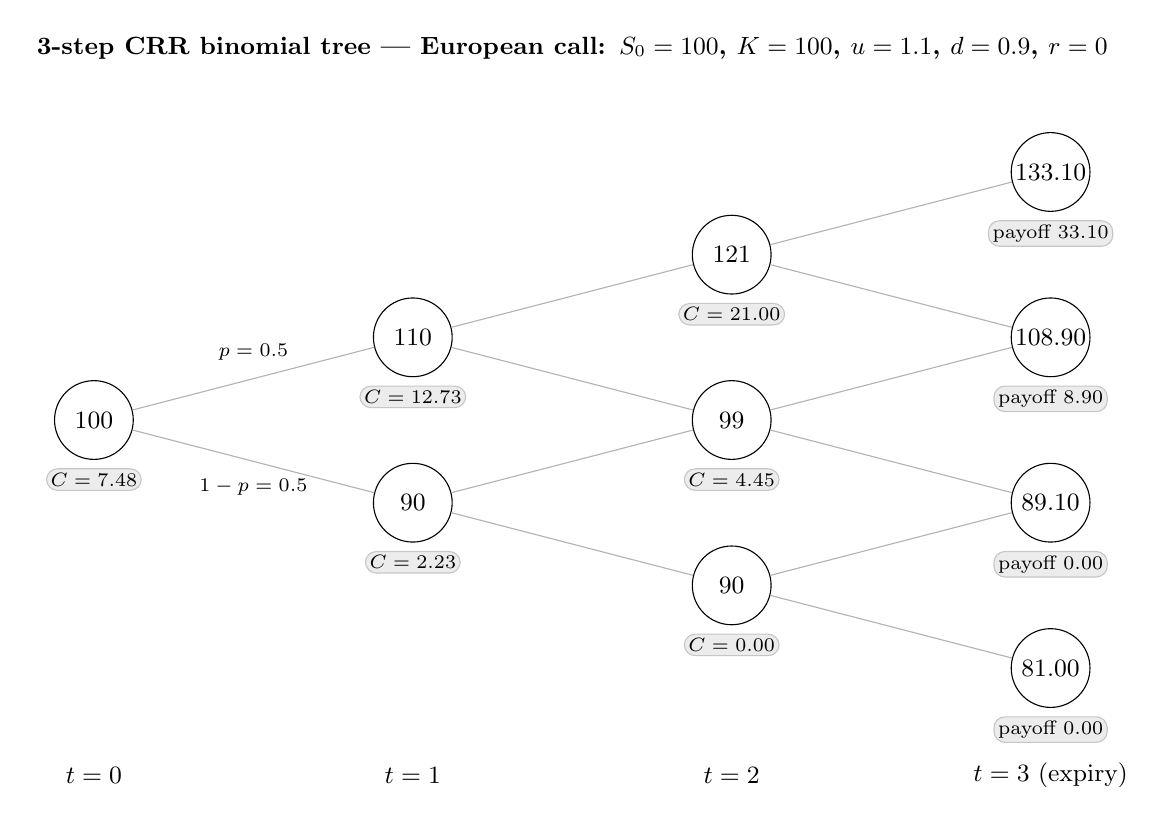
\begin{tikzpicture}[x=1.35cm, y=1.05cm,
  n/.style={circle, draw, minimum size=1.0cm, inner sep=0pt, font=\small},
  c/.style={rounded corners, fill=gray!15, draw=gray!45, font=\scriptsize, inner sep=1.5pt}]
  % stock nodes
  \node[n] (s0)   at (0,0)  {$100$};
  \node[n] (s1u)  at (3,1)  {$110$};
  \node[n] (s1d)  at (3,-1) {$90$};
  \node[n] (s2uu) at (6,2)  {$121$};
  \node[n] (s2ud) at (6,0)  {$99$};
  \node[n] (s2dd) at (6,-2) {$90$};
  \node[n] (s3uuu) at (9,3) {$133.10$};
  \node[n] (s3uud) at (9,1) {$108.90$};
  \node[n] (s3udd) at (9,-1) {$89.10$};
  \node[n] (s3ddd) at (9,-3) {$81.00$};
  % edges
  \foreach \from/\to in {s0/s1u, s0/s1d, s1u/s2uu, s1u/s2ud, s1d/s2ud, s1d/s2dd,
                     s2uu/s3uuu, s2uu/s3uud, s2ud/s3uud, s2ud/s3udd, s2dd/s3udd, s2dd/s3ddd}
    \draw[gray!60, thin] (\from) -- (\to);
  % prob labels
  \node[font=\scriptsize, above] at (1.5,0.6) {$p = 0.5$};
  \node[font=\scriptsize, below] at (1.5,-0.6) {$1-p = 0.5$};
  % option values
  \node[c, below=3pt of s0]   {$C = 7.48$};
  \node[c, below=3pt of s1u]  {$C = 12.73$};
  \node[c, below=3pt of s1d]  {$C = 2.23$};
  \node[c, below=3pt of s2uu] {$C = 21.00$};
  \node[c, below=3pt of s2ud] {$C = 4.45$};
  \node[c, below=3pt of s2dd] {$C = 0.00$};
  \node[c, below=3pt of s3uuu] {payoff $33.10$};
  \node[c, below=3pt of s3uud] {payoff $8.90$};
  \node[c, below=3pt of s3udd] {payoff $0.00$};
  \node[c, below=3pt of s3ddd] {payoff $0.00$};
  % step labels
  \node[font=\small] at (0,-4.3)  {$t=0$};
  \node[font=\small] at (3,-4.3)  {$t=1$};
  \node[font=\small] at (6,-4.3)  {$t=2$};
  \node[font=\small] at (9,-4.3)  {$t=3$ (expiry)};
  % title
  \node[font=\small\bfseries] at (4.5,4.5)
    {3-step CRR binomial tree — European call: $S_0 = 100$, $K = 100$, $u = 1.1$, $d = 0.9$, $r = 0$};
\end{tikzpicture}
\end{document}
